\documentclass[mathserif]{beamer}

\usepackage{microtype}
\usepackage{xparse}
\usepackage{siunitx}
\usepackage{graphicx}

% Typography and font packages.
\usepackage{lmodern}
\usepackage{microtype}

% Math packages.
\usepackage{amsmath}
\usepackage{amssymb}
\usepackage{mathtools}
\usepackage{commath}
\usepackage{siunitx}

\frenchspacing

% Macros for math
\newcommand{\such}{\mid}
\newcommand{\real}{\mathbb{R}}
\newcommand{\integer}{\mathbb{Z}}
\DeclarePairedDelimiter{\ceil}{\lceil}{\rceil}
\DeclarePairedDelimiter{\floor}{\lfloor}{\rfloor}

% Unit setup
\NewDocumentCommand{\varSI}{}{\SI[number-math-rm=\mathnormal,parse-numbers=false]} % Use variables as the value of units.


\logo{\includegraphics[width=0.07\textwidth]{../Logo}}

\sisetup{
	detect-all,
	math-rm=\mathrm,
	math-sf=\mathrm,
	math-tt=\mathrm
}

\usetheme{Rochester}
\usecolortheme{whale}

\setbeamertemplate{frametitle continuation}[from second][\hfill\insertcontinuationtext]

% Table of contents at start of each section
\AtBeginSection[] {%
	\begin{frame}
		\frametitle{Table of Contents}
		\tableofcontents[currentsection]
	\end{frame}
}

% Environments for math
\newenvironment{compactmath}[1][\normalsize]%
	{\begin{minipage}{\textwidth}\vspace{-0.5\baselineskip}#1\begin{equation*}}
	{\end{equation*}\end{minipage}}

\newenvironment{sizedmath}[1]%
	{\begingroup#1\begin{equation*}}
	{\end{equation*}\endgroup}

% Environments for consistent frame use
\newenvironment{namedframe}[1]%
	{\begin{frame}\frametitle{#1}\framesubtitle{\secname}}
	{\end{frame}}

\newenvironment{namedbreakframe}[1]%
	{\begin{frame}[allowframebreaks]\frametitle{#1}\framesubtitle{\secname}}
	{\end{frame}}

% Frames for emphasis
\newcommand{\sectionstart}[2]{\begin{frame}\frametitle{#1}\centering\Huge\secname\\\Large#2\end{frame}}
\newcommand{\bigframe}[1]{\begin{namedframe}{#1}\Huge\centering#1\end{namedframe}}

% Spacing commands
\newcommand{\sep}[1][1ex]{\\\pause\vspace{#1}}
\newcommand{\vsep}[1][1ex]{\pause\vspace{#1}}
\newcommand{\vertspace}[1][1ex]{\\\vspace{#1}}

% Do not use these, there are only for backwards compatibility with my old slides.
\newcommand{\varvertspace}[1]{\\\vspace{#1}}
\newcommand{\varsep}[1]{\\\pause\vspace{#1}}
\newcommand{\varvsep}[1]{\pause\vspace{#1}}

% Text formatting
\DeclareTextFontCommand{\emph}{\bfseries}


\usepackage{adjustbox}
\usepackage{wrapfig}
\usepackage{textpos}
\usepackage{tikz}
\usepackage{tkz-euclide}
\usetikzlibrary{angles,quotes}
\usetkzobj{all}

\title{Euclid Preparation 4}
\subtitle{Proofs}
\author{Lev Raizman}
\institute{William Lyon Mackenzie C.I. Math Club}
\date{\copyright{} Lev Raizman, 2018}

\begin{document}
	\frame{\titlepage}
	\section{Direct Proof}
	%\if{false}
	\begin{namedframe}{What is it?}
		A direct proof it the most basic type of proof.
		\sep
		It follows a set of logically true statements, which allow one to arrive from statement A to statement B.
		\sep
		They can rely on axioms, definitions, and earlier proved COMMON KNOWLEDGE theorems.
		\sep
		Proof by example is a sub-category of direct proofs, and is not covered in this lesson. It consists of finding a single case to a supposition in the form of ``There exists $N$ such that ...''.
	\end{namedframe}
	\subsection{Important Definitions}
\begin{namedframe}{Definitions}
	An integer $N$ is even if it can be expressed as $N=2M$ where $M$ is also an integer.
	\sep
	An integer $N$ is odd if it can be expressed as $N=2M+1$ where $M$ is also an integer.
	\pause
	Sometimes, $2M-1$ is used.
\end{namedframe}

	\subsection{Examples}
\begin{namedframe}{Odd Number Squared}
	\begin{example}
		Given an odd integer $N$, prove that $N^2$ is also an odd integer.	
	\end{example}
	\pause
	If $N$ is odd, it can be expressed as $2M-1$.
	\pause
	\begin{align*}
		\uncover<+->{N^2 &= (2M-1)^2\\}
		\uncover<+->{ &= 4M^2-4M+1\\}
		\uncover<+->{ &= 2(2M^2-4M)+1}
	\end{align*}
	\uncover<+->{
	Therefore $N^2$ is also odd.}	
\end{namedframe}
\begin{namedframe}{Pythagorean Theorem}
	\begin{example}
		Given a right angled triangle, the sum of the squares of the two legs is equal to the square of the hypotenuse.	
	\end{example}
	\begin{columns}
	\begin{column}{0.5\textwidth}
	\begin{tikzpicture}[scale = 0.5]
		\coordinate [label=below left:$A$](A) at (0,0);
		\coordinate [label=below right:$B$](B) at (4,0);
		\coordinate [label=above right:$C$](C) at (4,3);
		
		\draw (A) -- (B) -- (C) -- cycle;
		\draw (A) rectangle (4,-4)node [midway] {$b^2$};
		\draw (B) rectangle (7,3)node [midway] {$a^2$};
		\draw [rotate around={36.8:(A)}](A) rectangle (5,5) node [midway] {$c^2$};
	\end{tikzpicture}
	\end{column}
	\pause
	\begin{column}{0.5\textwidth}
		In Canada, this theorem is provided to students without proof, despite the fact that over 1000 different ones exist.
	\end{column}
	\end{columns}
\end{namedframe}
\begin{namedframe}{Pythagorean Theorem}
	\pause
	\begin{columns}
	\begin{column}{0.5\textwidth}
		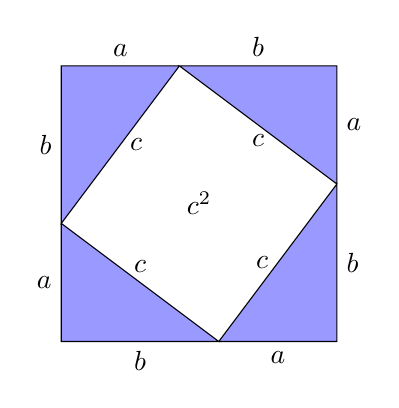
\begin{tikzpicture}[scale = 0.5]
		\coordinate (A) at (0,0);
		\coordinate (B) at (7,0);
		\coordinate (C) at (7,7);
		\coordinate (D) at (0,7);
		\coordinate (AB) at (4,0);
		\coordinate (BC) at (7,4);
		\coordinate (CD) at (3,7);
		\coordinate (DA) at (0,3);

		%\draw (A)rectangle(C) node [midway] {$c^2$};
		%\draw (A) -- node[below]{$b$}(AB) -- node[below]{$a$}(B);
		%\draw (B) -- node[right]{$b$}(BC) -- node[right]{$a$}(C);
		%\draw (C) -- node[above]{$b$}(CD) -- node[above]{$a$}(D);
		%\draw (D) -- node[left]{$b$}(DA) -- node[left]{$a$}(A);
		%\draw (AB) -- node[left]{$c$}(BC) -- node[below]{$c$}(CD) -- node[right]{$c$}(DA) -- node[above]{$c$}(AB) ; 
		\draw (3.5,3.5)node {$c^2$};
		
		\filldraw[fill=blue!40!white, draw=black] (DA) -- node[left]{$a$}(A) -- node[below]{$b$}(AB) -- node[above]{$c$}(DA);
		\filldraw[fill=blue!40!white, draw=black] (AB) -- node[below]{$a$}(B) -- node[right]{$b$}(BC) -- node[left]{$c$}(AB);
		\filldraw[fill=blue!40!white, draw=black] (BC) -- node[right]{$a$}(C) -- node[above]{$b$}(CD) -- node[below]{$c$}(BC);
		\filldraw[fill=blue!40!white, draw=black] (CD) -- node[above]{$a$}(D) -- node[left]{$b$}(DA) -- node[right]{$c$}(CD);
		\end{tikzpicture}
	\end{column}
	\pause
	\begin{column}{0.5\textwidth}
		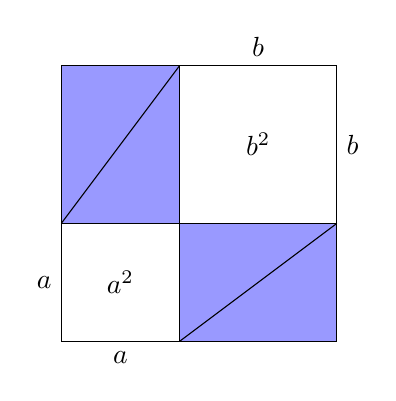
\begin{tikzpicture}[scale = 0.5]
		\coordinate (A) at (0,0);
		\coordinate (B) at (7,0);
		\coordinate (C) at (7,7);
		\coordinate (D) at (0,7);
		\coordinate (AB) at (3,0);
		\coordinate (BC) at (7,3);
		\coordinate (CD) at (3,7);
		\coordinate (DA) at (0,3);
		
		\filldraw[fill=blue!40!white, draw=black]  (AB) rectangle (BC);
		\filldraw[fill=blue!40!white, draw=black]  (CD) rectangle (DA);
		\draw (AB) -- (BC);
		\draw (CD) -- (DA);
		\draw (DA) -- node[left]{$a$}(A) -- node[below]{$a$}(AB);
		\draw (BC) -- node[right]{$b$}(C) -- node[above]{$b$}(CD);
		
		\draw (1.5,1.5)node {$a^2$};
		\draw (5,5)node {$b^2$};
		%\filldraw[fill=blue!40!white, draw=black]  (CD) -- (D) -- (DA) -- (CD);
		%\filldraw[fill=blue!40!white, draw=black]  (AB) -- (B) -- (BC) -- (AB);
		\end{tikzpicture}
	\end{column}
	\end{columns}
\end{namedframe}
	%\fi
	\section{Proof by Contradiction}
	%\if{false}
	\begin{namedframe}{What is it?}
		A proof by contradiction is another common method of proving a statement.
		\sep
		It makes an assumption, and then follows through a set of logical steps that show that if the assumption is true, the assumption must be false. This results in a contradiction, meaning the assumption is false.
		\sep
		A similar style of proof is called ``Proof by Contraposition'', which proves a statement ``If $A$ then $B$'' by proving that ``If not $A$, then not $B$''.
	\end{namedframe}
	\subsection{Examples}
\begin{namedframe}{Odd Number Squared}
	\begin{example}
		Given an odd integer $N^2$, prove that $N$ must be an odd integer.	
	\end{example}
	\pause
	Suppose that $N$ is not an odd integer. Thus, it can be expressed as $2M$.
	\pause
	\begin{align*}
		\uncover<+->{N^2 &= (2M)^2\\}
		\uncover<+->{ &= 4M^2\\}
		\uncover<+->{ &= 2(2M^2)}
	\end{align*}
	\uncover<+->{
		$N^2$ is not odd. Therefore, $N$ \textit{is not} not an odd integer, and must be odd.
	}
\end{namedframe}
\begin{namedframe}{Irrationality of $\sqrt{2}$}
	Legend goes that Pythagoras drowned the student that proved the existence of irrational numbers.\pause Quite irrational of him! \pause Moreover, it is believed that the proof of the existence of irrational numbers was done using $\sqrt{2}$. It has also become the classical proof by contradiction.
	\pause
	\begin{example}
		Prove that $\sqrt{2}$ is irrational.	
	\end{example}
	Let's assume that $\sqrt{2}$ is rational.\pause Then, it can be expressed as $\frac{a}{b}$ where $a$ and $b$ are integers and have no common factors. If they have common factors, divide both by the factor until the original condition is met. This has been shown to be possible for any two integers in an earlier lesson.
\end{namedframe}
\begin{namedframe}{Irrationality of $\sqrt{2}$}
	\vspace{-.5cm}
	\begin{align*}
		\uncover<+->{\sqrt{2} &= \frac{a}{b}\\}
		\uncover<+->{\sqrt{2}b &= a\\}
		\uncover<+->{2b^2 &= a^2\\}
	\end{align*}
	
	\uncover<+->{This means that $a$ is even, and can be expressed as $2c$.}
	\begin{align*}
		\uncover<+->{2b^2 &= (2c)^2\\}
		\uncover<+->{b^2 &= 2c^2\\}
	\end{align*}
	\uncover<+->{As before, the above statement implies that $b$ is even.} 	\uncover<+->{However, if both $a$ and $b$ are even, then they share a common factor 2. This contradicts the original assumption. Therefore, $\sqrt{2}$ is irrational.}
\end{namedframe}
	%\fi
	\section{Proof by Exhaustion}
	%\if{false}
	\begin{namedframe}{What is it?}
		This proof is a case by case proof, but must be used with caution.
		\sep
		It splits the question into all the possible cases, and then proves that the statement is true for all possible cases.
		\sep
		It can look very disorganized, especially if the cases are singular numbers instead of sets, but it is still a proof.
	\end{namedframe}
	\subsection{Examples}
\begin{namedframe}{Odd Number Squared}
	\begin{example}
		Given an integer $N$, prove that $N^2$ must be even, or one greater than even.*	
	\end{example}
	\pause
	Separate the problem into two cases: $N$ is odd, or $N$ is even. Then, you will find that one case will yield an even number (namely $N$ is even) and the other case will yield a number one greater than even (namely $N$ is odd).
\end{namedframe}
\begin{namedframe}{Actual Example}
	\begin{example}
		Given a perfect cube $N^3$, prove that it is always divisible by 9, or 1 greater or 1 less than that.
	\end{example}
	\pause
	For this problem, we will make 3 cases: $N$ is divisible by 3, $N$ is one less than a number divisible by 3, and $N$ is one greater than a number divisible by 3.
\end{namedframe}
\begin{namedframe}{Case 1}
	Case 1 ($N$ is divisible by 3, and can be expressed as $3M$):
	\pause
	\begin{align*}
		N^3 &= (3M)^3\\
			&= 27M^3\\
			&= 9(3M^3)
	\end{align*}
\end{namedframe}
\begin{namedframe}{Case 2}
	Case 2 ($N$ is one less than a number divisible by 3, and can be expressed as $3M-1$):
	\pause
	\begin{align*}
		N^3 &= (3M-1)^3\\
		&= 27M^3-27M^2+9M-1\\
		&= 9(3M^3-9M^2+M)-1
	\end{align*}
\end{namedframe}
\begin{namedframe}{Case 3}
	Case 3 ($N$ is one greater than a number divisible by 3, and can be expressed as $3M+1$):
	\pause
	\begin{align*}
		N^3 &= (3M+1)^3\\
		&= 27M^3+27M^2+9M+1\\
		&= 9(3M^3+9M^2+M)+1
	\end{align*}
\end{namedframe}
\begin{namedframe}{Conclusion}
	The three cases are \textit{exhaustive} (cover all possibilities), and the result fits the conjecture. Therefore, the statement is true.
\end{namedframe}
	%\fi
	\section{Nonconstructive Proof}
	%\if{false}
	\begin{namedframe}{What is it?}
		This proof is quite rare, and is somewhat similar to an exhaustive proof
		\sep
		It relies on showing that within a given set of parameters something must be possible, without pinpointing exactly what it is. This is why it is called nonconstructive.It also often relies on exhaustive properties of these parameters.
		\sep
		It is also sometimes called ``Proof by Ternary Exclusion'', when there are two cases, and no third one is possible.
	\end{namedframe}
	\subsection{Examples}
\begin{namedframe}{Odd Number Squared}
	\begin{example}
		Given an integer $N$, prove that $N^2$ must be even, or one greater than even.*	
	\end{example}
	\pause
	This problem can be solved non-constructively. Simply noting that every number is either even, or one greater than even (odd), proves that this must be true. This is a nonconstructive proof because you proved the statement without finding the exact answer. A better example follows.
\end{namedframe}
\begin{namedframe}{Irrational to the Irrational}
	\begin{example}
		Prove that it is possible to have an irrational number to the power of another irrational number result in a rational number.
	\end{example}
	\pause
	Recall that $\sqrt{2}$ is irrational. Let us consider two cases: $\sqrt{2}^{\sqrt{2}}$ and $(\sqrt{2}^{\sqrt{2}})^{\sqrt{2}}$. \sep If the first case is rational, then we have found an example to match the statement.\sep If it is not rational, it must be irrational. This is the exhaustive part.\pause However, simplifying the second case allows one to see that the result is 2.\sep One of the two cases must be an irrational to the power of an irrational resulting in a rational. However, the specific one is unknown. This is the nonconstructive part.
\end{namedframe}
	%\fi
	\section{Proof by Induction}
	%\if{false}
	\begin{namedframe}{What is it?}
		This proof is extremely versatile, and should be applied if possible.
		\sep
		It relies on proving a case, then assuming that the statement is true, and proving that the statement is always true for an input one greater or one less. This results in a recursive proof of all other values.
		\sep
		Despite its name, the proof is still deductive, not inductive.
	\end{namedframe}
	\subsection{Examples}
\begin{namedframe}{Odd Number Squared}
	\begin{example}
		Given an odd integer $N$, prove that $N^2$ is also an odd integer.	
	\end{example}
	\pause
	First, check that it is true for $N=1$.
	\pause
	\begin{align*}
		N^2 &= 1^2\\
			&= 1
	\end{align*}
\end{namedframe}
\begin{namedframe}{Odd Number Squared}
	Next, assume that it is true for all $N$. Now prove that it is true for any $N+2$. It cannot be for $N+1$, because an odd number plus 1 is even, while the proof asks for odd. Recall that if $N$ is odd, it can be expressed as $2M+1$.
	\begin{align*}
		(N+2)^2 &= (2M+3)^2\\
			&= 2M^2+12M+9\\
			&= 2(M^2+6M+4)+1\\
	\end{align*}
	\pause
	Therefore, any $N+2$ is also odd.\pause This works because we showed that the statement is true for $N=1$. From the above, we know that it is also true for $N+2$, in this case 3. However, this implies that it is also true for 5, which in turn implies that it is true for 7, and so on until all odd integers are covered.
\end{namedframe}
\begin{namedframe}{Arithmetic Sequence}
	\begin{example}
		Prove that $p(N)=0+1+2+3+...+N-1+N=\frac{N(N+1)}{2}$.
	\end{example}
	First, check that it is true for $N=0$.
	\pause
	\begin{align*}
		0 &= \frac{0(0+1)}{2}\\
		&= 0
	\end{align*}
	\pause
	Assume it is true from p(N). Now prove that it is true for p(N+1).
\end{namedframe}
\begin{namedframe}{Inductive Portion}
	\begin{block}{What is being proven!}
		\centering$0+1+2+..+N+(N+1) = \frac{(N+1)((N+1)+1)}{2}$
	\end{block}
	\begin{align*}
		\uncover<+->{0+1+2+..+N+(N+1) &= \frac{N(N+1)}{2} + (N+1)\\}
		\uncover<+->{&= \frac{N(N+1)+2(N+1)}{2}\\}
		\uncover<+->{&= \frac{(N+2)(N+1)}{2}\\}
		\uncover<+->{&= \frac{(N+1)((N+1)+1)}{2}\\}
	\end{align*}
	\uncover<+->{Which is what needed to be proven. $Q.E.D.$}
\end{namedframe}
\begin{namedframe}{Addition and Subtraction when Inducing}
	\begin{example}
		Prove that $4^N-1$ is always divisible by 3 if $N$ is a positive integer.
	\end{example}
	First, check that the statement is true for $N=1$.
	\begin{align*}
		4^N-1 &= 4^1-1\\
		&= 3\\
	\end{align*}
	Assume it is true for $N$, now prove for $N+1$.\pause This time, we will take the difference between the statement for $N$ and $N+1$. Because the statement is assumed to be true for $N$, if their difference is divisible by 3, then it must also be divisible by 3 for $N+1$.
\end{namedframe}
\begin{namedframe}{Addition and Subtraction when Inducing}
	\begin{align*}
	\uncover<+->{4^{N+1}-1 - (4^N-1)&= 4^{N+1}-4^N\\}
	\uncover<+->{&= 4^N(4^1-1)\\}
	\uncover<+->{&= 4^N(3)\\}
	\end{align*}
	\uncover<+->{Thus, the statement is true.}
\end{namedframe}
	%\fi
\end{document}